%HELPFULL TROUBLESHOOT PAGES
% www.google.com
% https://www.overleaf.com/learn
% https://www.overleaf.com/learn/latex/Multiple_columns
% https://www.overleaf.com/learn/latex/Using_colours_in_LaTeX
\documentclass[8pt,usenames,dvipsnames,twoside]{article}
%-----------------------------------------------------------------
% FORMATTING
%-----------------------------------------------------------------
% all formatting and packages are in this file
\input{./format/checklistformat_20210301}

%-----------------------------------------------------------------
% BEGIN DOCUMENT
%-----------------------------------------------------------------
\title{F14_Cheatsheet}
% apply hatching to all pages
\AtBeginShipout{\AtBeginShipoutAddToBox{\Hatch}}
\begin{document}
	%-----------------------------------------------------------------
% TITLE PAGE
%-----------------------------------------------------------------
	% deactivate header and footer
	\pagestyle{empty}
	\newlength{\centeroffset}
	\setlength\centeroffset{(\chevin-\outmar-0.5cm)/2}
	\begin{tikzpicture}[overlay, remember picture]
	\node[
	]() at ([xshift=\centeroffset,yshift=8.5cm]current page.center) {
		\Huge \textbf{Pocket Checklist} 
	};
	\node[
	]() at ([xshift=\centeroffset,yshift=7cm]current page.center) {
		\resizebox{10cm}{!}{\textbf{\colorbox{black}{\textcolor{white}{F-14A/B AIRCRAFT}}}}
	};
	\node[
	]() at ([xshift=\centeroffset,yshift=5.5cm]current page.center) {
		\Large \textbf{\colorbox{color1}{\textcolor{white}{REV: \today}}} \blue{}
	};
	\node[
	]() at ([xshift=\centeroffset,yshift=-1cm]current page.center) {
		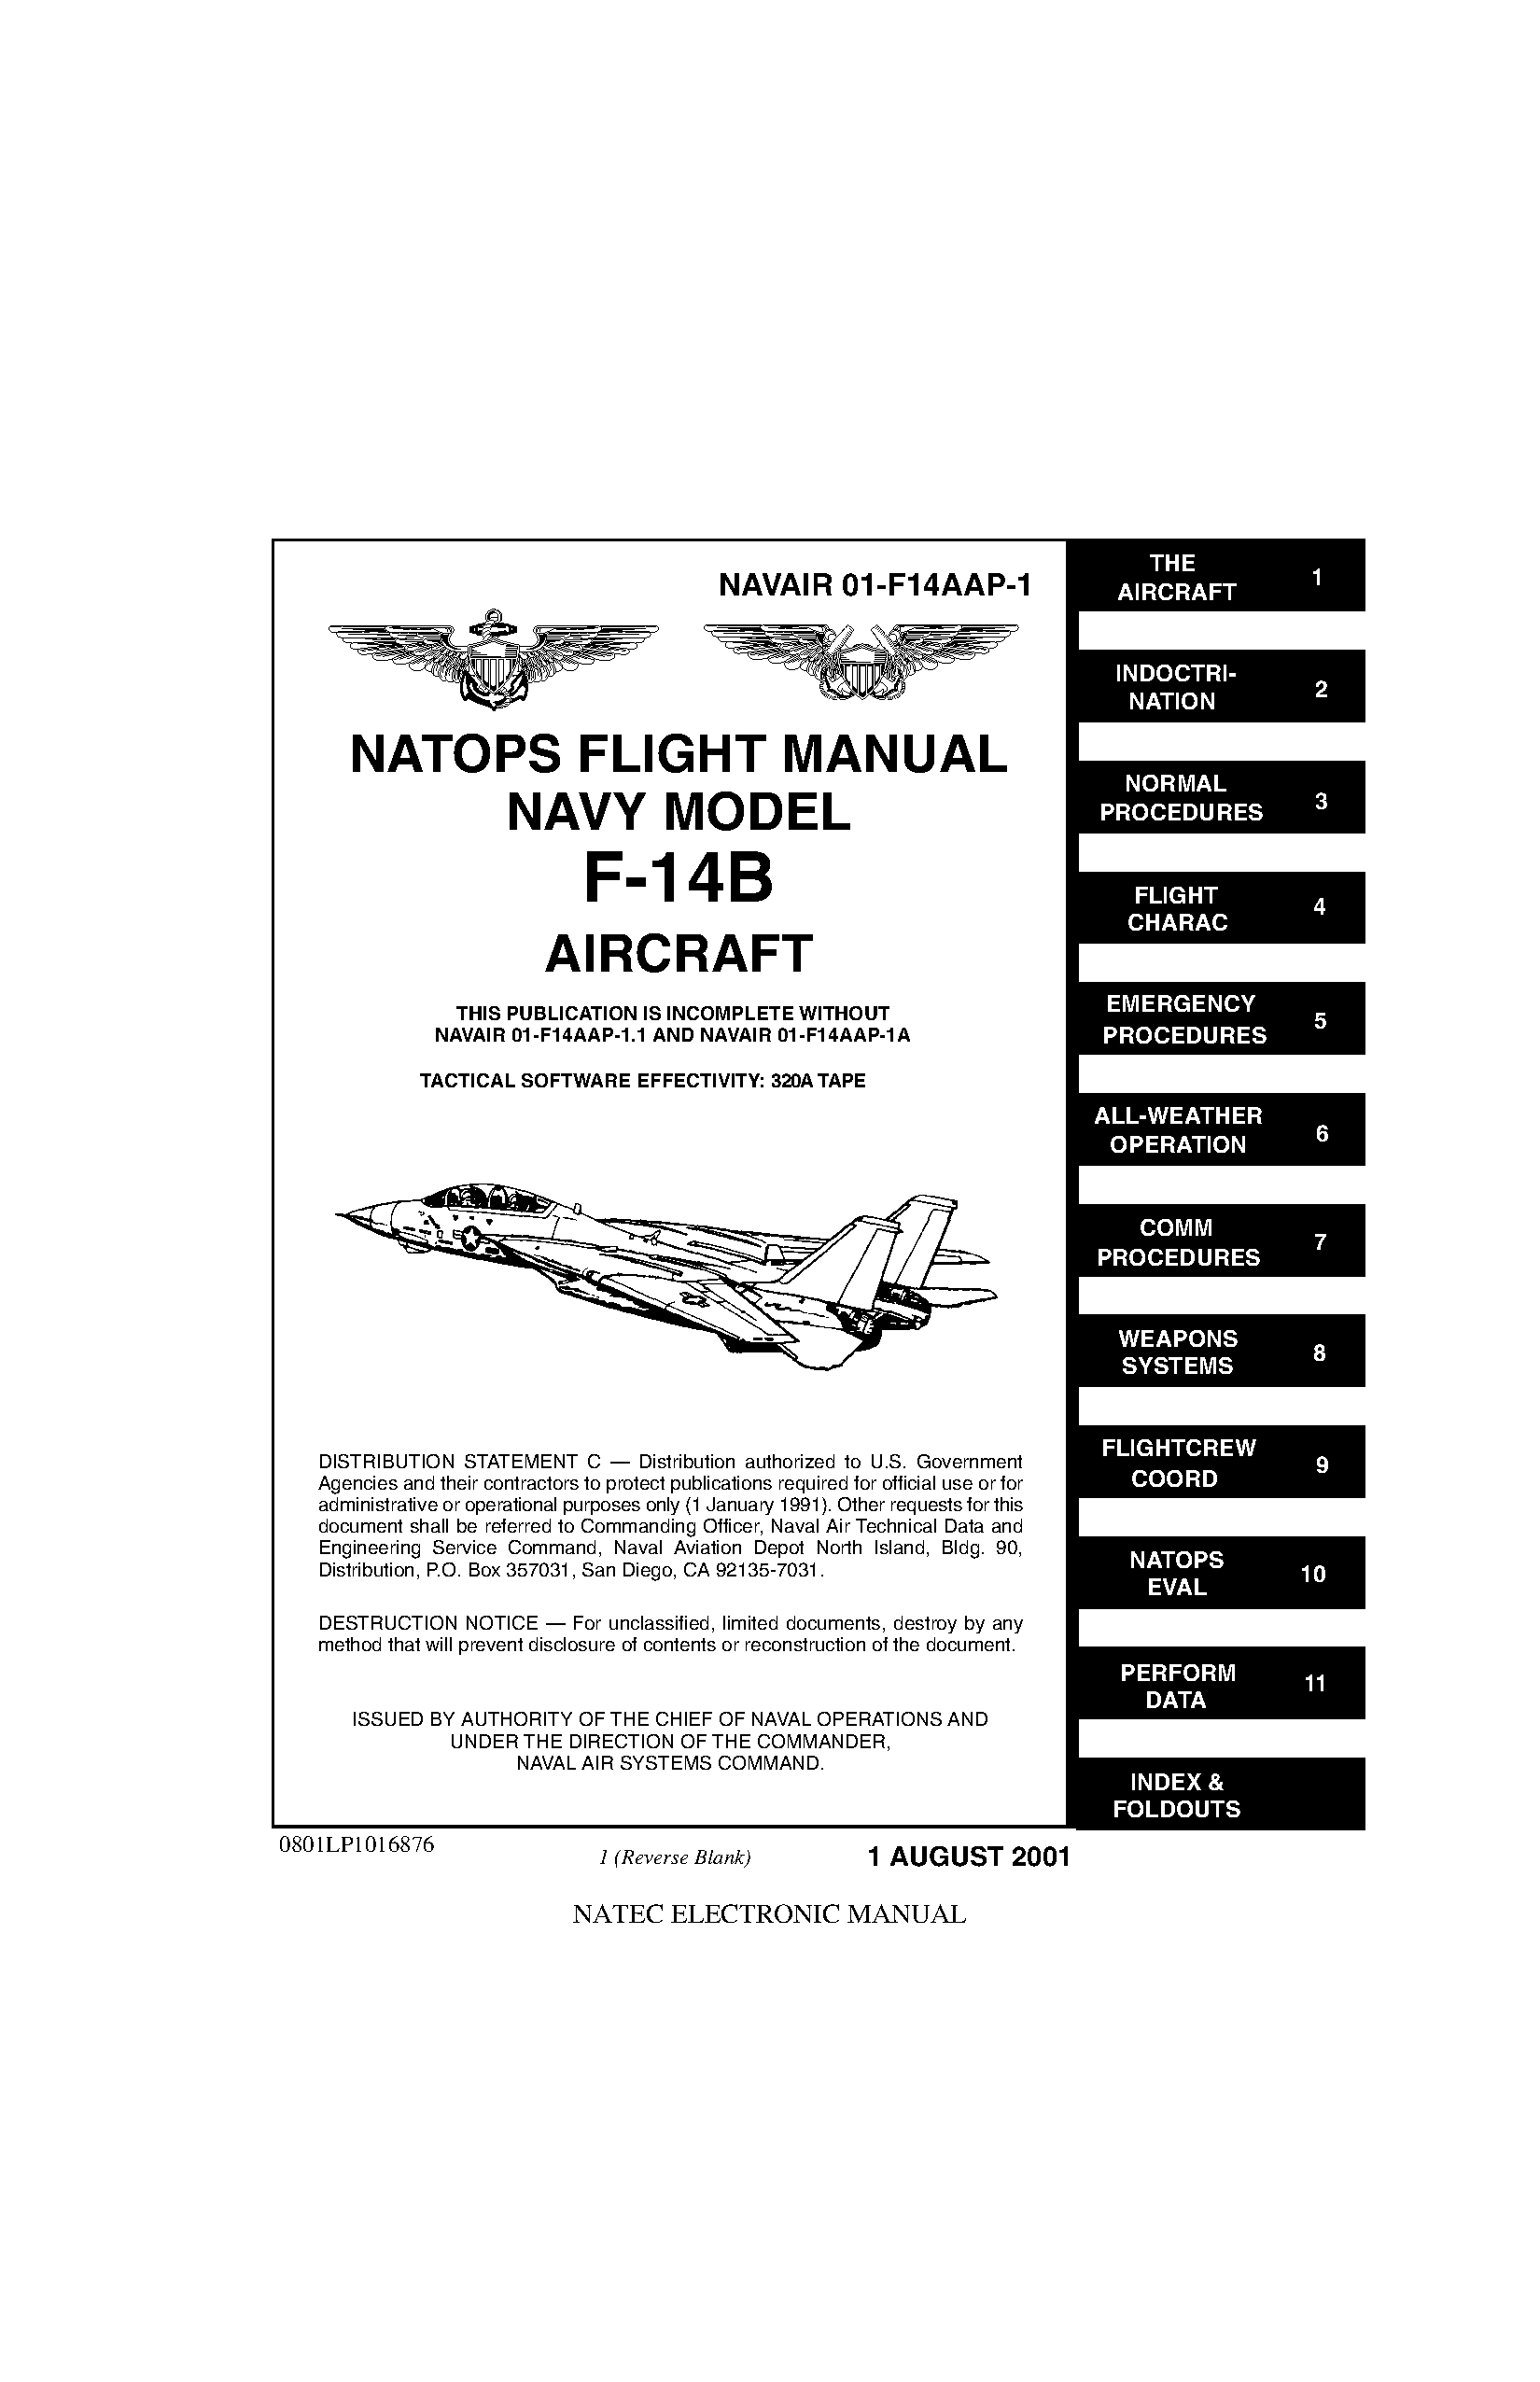
\includegraphics[
			width=0.8\linewidth,
			page = {1},
			trim = {3cm, 10.5cm, 6.5cm, 13.5cm},
			clip
		]{natops_F14B.pdf}
	};
	% Black area for white chevrons
	\fill[black]
		([xshift=\outmar, yshift=0.2cm]current page text area.north east) -- 
		([xshift=\outmar, yshift=-\botmar]current page text area.south east) -- 
		([xshift=\chevin-0.5cm, yshift=-\botmar]current page text area.south east) -- 
		([xshift=\chevin-0.5cm, yshift=0.2cm]current page text area.north east) -- 
		cycle;
	\end{tikzpicture}
	% label for hyperrefs back to frontpage
	\label{frontpage}
	% make chevrons
	\thumbfront{Procedures}{0}
	\thumbfront{Systems}{1}
	% use tabular for multi line node
	\thumbfront{\begin{tabular}{c} AWG-9 \\ Radar \end{tabular}}{2}
	\thumbfront{\begin{tabular}{c} TCS \\ ALQ-100 \end{tabular}}{3}
	\thumbfront{\begin{tabular}{c} LANTIRN \end{tabular}}{4}
	\thumbfront{\begin{tabular}{c} A/G \\ Weapons \end{tabular}}{5}
	\thumbfront{\begin{tabular}{c} A/A \\ Weapons \end{tabular}}{6}
	\thumbwide
	\cleardoublepage
	
	\thumbnar
	\tableofcontents
	\cleardoublepage
	
	% restart page counter
	\setcounter{page}{1}
	% reactivate header and footer
	\pagestyle{plain}
	
		\section{PROCEDURES}
		\thumbtab{Procedures}{0}
		
		\subsection{PILOT - PRE-START}
		\begin{center}
			\begin{longtable}{l p{3cm} | p{7cm}}
				\toprule
				1. & \blue{Parking Break} & \textbf{ENGAGED} \\
				\midrule
				2. & \blue{Ground Power} & connected \\
				\midrule
				3. & \blue{Compressed Air} & connected \\
				\midrule
				4. & \blue{ICS} & \textbf{HOT MIC} \\
				\midrule
				5. & \dblue{TO RIO} & \emph{``Begin Start-Up''} \\
				\midrule
				6. & \blue{ICS} & \textbf{Comm Check} \\
				\midrule
				7. & \blue{MASTER TEST Selector} & 
				\begin{minipage}[t]{\linewidth}
					\vspace{-7pt}
					\begin{enumerate}[label=(\alph*)]
						\item \textbf{LTS}
						\begin{itemize}
							\item \textbf{Warning Lights} \dotfill checked
							\item \textbf{Caution Lights} \dotfill checked
							\item \textbf{Advisory Lights} \dotfill checked
						\end{itemize}
						\item \textbf{FIRE DET/EXT}
						\begin{itemize}
							\item \textbf{L FIRE GO} \dotfill illuminated
							\item \textbf{R FIRE GO} \dotfill illuminated
						\end{itemize}
						\item \textbf{INST}
						\begin{itemize}
							\item \textbf{RPM} \dotfill 96\%
							\item \textbf{EGT} \dotfill 960 C
							\item \textbf{FF} \dotfill 10500 pph
							\item \textbf{AOA} \dotfill 18 $\pm$ 5
							\item \textbf{Wing Sweep} \dotfill 45 $\pm$ 2.5
							\item \textbf{FUEL QT}Y \dotfill 2000 $\pm$ 200 
							\item \textbf{Oxygen QTY} \dotfill 2 liters
							\item \textbf{L\&R FF lights} \dotfill illuminated
						\end{itemize}
						\item \textbf{OFF}
					\end{enumerate}
				\end{minipage} \\
				\midrule
				8. & \blue{Ejection Seat} & Armed \\
				\midrule
				9. & \dblue{RIO} & Canopy Closed \\
				\midrule
				10. & \blue{Oxygen} & \textbf{ON (FWD)} \\
				\midrule
				11 & \blue{Emergency Wing Sweep} & \textbf{OVERSWEEP} \\
				\bottomrule
			\end{longtable}
		\end{center}
		\clearpage
		
		\subsection{PILOT - ENGINE START}
		\begin{center}
			\begin{longtable}{l p{3cm} | p{7cm}}
				\toprule
				1. & \blue{AIR SOURCE} & \textbf{OFF} \\
				\midrule
				2. & \blue{Hydraulics} & 
				\begin{minipage}[t]{\linewidth}
					\vspace{-7pt}
					\begin{enumerate}[label=(\alph*)]
						\item \textbf{HYD TRANSFER PUMP} \dotfill \textbf{SHUTOFF}
						\item \textbf{Emerg. Hyd.} \dotfill \textbf{AUTO (LOW)} 
					\end{enumerate}
				\end{minipage} \\
				\midrule
				3. & \blue{L\&R MASTER GEN} & \textbf{NORM} \\
				\midrule
				4. & \dblue{RIO} & \emph{``Ready to Start''} \\
				\midrule
				5. & \blue{Right Engine Start-Up} & 
				\begin{minipage}[t]{\linewidth}
					\vspace{-7pt}
					\begin{enumerate}[label=(\alph*)]
						\item \textbf{Engine Crank} \dotfill \textbf{R} 
						\item \textbf{R Eng N2} \dotfill 20\%
						\item \textbf{R Throttle} \dotfill \textbf{IDLE} 
						\item \textbf{TIT} \dotfill < 890 C during start
						\item \textbf{R GEN CAUTION} \dotfill extinguished
					\end{enumerate}
				\end{minipage} \\
				\midrule
				6. & \blue{Stabilized Parameters} & 
				\begin{minipage}[t]{\linewidth}
					\vspace{-7pt}
					\begin{itemize}
						\item \textbf{RPM} \dotfill 62-78\%
						\item \textbf{TIT} \dotfill approx 500 C
						\item \textbf{Fuel Flow} \dotfill 950-1400 pph
						\item \textbf{NOZ} \dotfill 5 (100\%)
						\item \textbf{Oil Pressure} \dotfill 25-35 psi
						\item \textbf{Hyd Pressure} \dotfill 3000 psi
					\end{itemize} 
				\end{minipage} \\
				\midrule
				7. & \blue{Left Engine Start-Up} & 
				\begin{minipage}[t]{\linewidth}
					\vspace{-7pt}
					\begin{enumerate}[label=(\alph*)]
						\item \textbf{Engine Crank} \dotfill \textbf{L} 
						\item \textbf{L Eng N2} \dotfill 20\%
						\item \textbf{L Throttle} \dotfill \textbf{IDLE} 
						\item \textbf{TIT} \dotfill < 890 C during start
						\item \textbf{L GEN Caution} \dotfill extinguished
					\end{enumerate}
				\end{minipage} \\
				\midrule
				8. & \blue{Stabilized Parameters} & 
				\begin{minipage}[t]{\linewidth}
					\vspace{-7pt}
					\begin{itemize}
						\item \textbf{RPM} \dotfill 62-78\%
						\item \textbf{TIT} \dotfill approx 500 C
						\item \textbf{Fuel Flow} \dotfill 950-1400 pph
						\item \textbf{NOZ} \dotfill 5 (100\%)
						\item \textbf{Oil Pressure} \dotfill 25-35 psi
						\item \textbf{Hyd Pressure} \dotfill 3000 psi
					\end{itemize} 
				\end{minipage} \\
				\midrule
				9. & \blue{HYD TRANSFER PUMP} & \textbf{NORM} \\
				\midrule
				10. & \blue{HYD PRESSURE} & 3000 psi \\
				\midrule
				11. & \blue{AIR SOURCE} & \textbf{BOTH ENG} \\
				\midrule
				12. & \blue{Ground Power} & disconnected \\
				\midrule
				13. & \blue{Compressed Air} & disconnected \\
				\bottomrule
			\end{longtable}
		\end{center}
		
		\subsection{PILOT - POST-START}
		\begin{center}
			\begin{longtable}{l p{3cm} | p{7cm}}
				\toprule
				1. & \dblue{TO RIO} & \emph{``Both Engines Running''} \\
				\midrule
				2. & \blue{Displays Control Panel} &
				\begin{minipage}[t]{\linewidth}
					\vspace{-7pt}
					\begin{itemize}
						\item \textbf{VDI} \dotfill \textbf{ON}
						\item \textbf{HUD} \dotfill \textbf{ON}
						\item \textbf{HSD} \dotfill \textbf{ON}
						\item \textbf{HDS MODE} \dotfill \textbf{TID}\\
						\hfill (monitor INS)
					\end{itemize} 
				\end{minipage} \\
				\midrule
				3. & \dblue{RIO} & \textbf{Select Align Quality}
				\begin{minipage}[t]{\linewidth}
					\vspace{-7pt}
					\begin{itemize}
						\item \blue{INS GO NOW:} shortest but least precise alignment
						\item \blue{INS GO COARSE:} does not meet Launch Criteria for AIM-7 / AIM-54
						\item \blue{INS GO MIN WPN LAUNCH:} allows AIM-7 / AIM-54 launch
						\item \blue{INS GO FINE} fine align (8 min)
					\end{itemize} 
				\end{minipage} \\
				\midrule
				4. & \blue{ACM Panel} & 
				\begin{minipage}[t]{\linewidth}
					\vspace{-7pt}
					\begin{itemize}
						\item \blue{GUN RATE} \dotfill as required
						\item \blue{SW COOL} \dotfill \textbf{OFF}
						\item \blue{MSL PREP} \dotfill \textbf{OFF}
						\item \blue{Missile MODE/STP} \dotfill \textbf{NORM}
					\end{itemize} 
				\end{minipage} \\
				\midrule
				5. & \blue{Gun Rounds} & \textbf{Set} \\
				\midrule
				6. & \blue{ANTI-SKID SPOILER BK} & \textbf{OFF} \\
				\midrule
				7. & \blue{Emergency Wing Sweep} &
				\begin{minipage}[t]{\linewidth}
					\vspace{-7pt}
					\begin{enumerate}[label=(\alph*)]
						\item \blue{Handle} \dotfill \textbf{AFT}
						\item \blue{Angle} \dotfill Verify 68 deg
					\end{enumerate} 
				\end{minipage} \\
				\midrule
				8. & \blue{AFCS Panel - SAS STAB AUG} & 
				\begin{minipage}[t]{\linewidth}
					\vspace{-7pt}
					\begin{itemize}
						\item \blue{PITCH} \dotfill \textbf{ON}
						\item \blue{ROLL} \dotfill \textbf{ON}
						\item \blue{YAW} \dotfill \textbf{ON}
					\end{itemize} 
				\end{minipage} \\
				\midrule
				9. & \blue{WING/EXT TRANS} & \textbf{AUTO} \\
				\midrule
				10. & \blue{UHF 1 Function Selector} & \textbf{BOTH} \\
				\midrule
				11. & \blue{TACAN Function Selector} & \textbf{T/R} \\
				\midrule
				12. & \blue{ARA-63 ICLS RECEIVER} & \textbf{ON} \\
				\midrule
				13. & \blue{Radar Altimeter} & 
				\begin{minipage}[t]{\linewidth}
					\vspace{-7pt}
					\begin{enumerate}[label=(\alph*)]
						\item \blue{Control Knob} \dotfill one click CW to turn on
						\item \blue{Display} \dotfill 6000 ft (warm up) 
						\item \blue{Display} \dotfill 0 ft (ready)
					\end{enumerate} 
				\end{minipage} \\
				\midrule
				14. & \blue{Standby ADI} & erect at least 2 min before T/O \\
				\midrule
				15. & \blue{KY-28 Crypt. Key} & \textbf{Set} (refer to GROUND SETTINGS kb) \\
				\midrule
				16. & \dblue{RIO} & set D/L frequency \\
				\midrule
				17. & \blue{Lights} & As desired \\
				\bottomrule
			\end{longtable}
		\end{center}
	
		\cleardoublepage
		
		\thumbnar
		\subsection{RIO - PRE-START}
		\begin{center}
			\begin{longtable}{l p{3cm} | p{7cm}}
				\toprule
				1. & \blue{Oxygen} & \textbf{ON (FWD)} \\
				\midrule
				2. & \dblue{PILOT} & 
				\begin{minipage}[t]{\linewidth}
					\vspace{-7pt}
					\begin{itemize}
						\item \textbf{Ground Power} \dotfill connected
						\item \textbf{Compressed Air} \dotfill connected
					\end{itemize} 
				\end{minipage} \\
				\midrule
				3. & \blue{ICS} & Comm Check \\
				\midrule
				4. & \blue{Lights} & As required \\
				\midrule
				5. & \blue{LTS Test} & Coordinate with Pilot \\
				\midrule 
				6. & \blue{Ejection Seats} & \textbf{ARMED} \\
				\midrule
				7. & \blue{Canopy} & \textbf{CLOSED} \\
				\midrule
				8. & \dblue{TO PILOT} & \emph{``Ready to Start''} \\
				\bottomrule
			\end{longtable}
		\end{center}
	
		\subsection{RIO - POST-START - SHORE}
		\begin{center}
			\begin{longtable}{l p{3cm} | p{7cm}}
				\toprule
				1. & \dblue{PILOT} & 
				\begin{minipage}[t]{\linewidth}
					\vspace{-7pt}
					\begin{itemize}
						\item \textbf{Engines} \dotfill started
						\item \textbf{AIR SOURCE} \dotfill BOTH ENG
					\end{itemize} 
				\end{minipage} \\
				\midrule
				2. & \blue{INS STARTUP} & 
				\begin{minipage}[t]{\linewidth}
					\vspace{-7pt}
					\begin{enumerate}[label=(\alph*)]
						\item \textbf{LIQUID COOLING} \dotfill \textbf{ON (FWD)}
						\item \textbf{WCS Switch} \dotfill \textbf{STANDBY}
						\item \textbf{IR/TV Power} \dotfill \textbf{STBY/IR/TV}
						\item \textbf{TID/DDD} \dotfill illuminated after 40 s
					\end{enumerate} 
				\end{minipage} \\
				\midrule
				3. & \blue{Kneeboard} & Retrieve Coordinates, Elevation, Magnetic Variation from GROUND SETTINGS Page \\
				\midrule
				\multicolumn{3}{l}{\blue{WARNING} Input Coords \textbf{BEFORE} selecting \textbf{GND ALIGN} if using ASH} \\
				\midrule
				4. & \blue{Start INS Align} & 
				\begin{minipage}[t]{\linewidth}
					\vspace{-7pt}
					\begin{enumerate}[label=(\alph*)]
						\item \blue{Nav Mode} \dotfill \textbf{GND ALIGN}
						\item \blue{CAP} 
						\begin{itemize}
							\item \textbf{Category} \dotfill \textbf{NAV}
							\item \textbf{MESSAGE} \dotfill \textbf{OWN AC}
						\end{itemize}
						\item \blue{Keyboard} 
						\begin{itemize}
							\item \textbf{CLEAR}, \textbf{LAT}, latitude, \textbf{ENTER}
							\item \textbf{LONG}, longitude, \textbf{ENTER}
							\item \textbf{ALT}, altitude, \textbf{ENTER}
						\end{itemize} 
						\item \blue{CAP MESSAGE} \dotfill \textbf{MAG HDG VAR}
						\item \blue{Keyboard} \dotfill \textbf{HDG}, mag var, \textbf{ENTER}
						\item \blue{Alignment Progress} \dotfill Monitor
					\end{enumerate} 
				\end{minipage} \\
				\midrule
				5. & \blue{U/VHF Mode} & \textbf{T/R G} \\
				\midrule
				6. & \blue{Datalink} & 
				\begin{minipage}[t]{\linewidth}
					\vspace{-7pt}
					\begin{enumerate}[label=(\alph*)]
						\item \blue{Kneeboard} \dotfill TACTICAL DL
						\item \blue{DL Power} \dotfill \textbf{ON (FWD)}
						\item \blue{DL Mode} \dotfill \textbf{TAC (AFT)}
						\item \blue{DL Freq.} \dotfill \textbf{Set}
					\end{enumerate} 
				\end{minipage} \\
				\midrule
				7. & \blue{TACAN} & \textbf{T/R} \\
				\midrule
				8. & \blue{RWR Panel} & 
				\begin{minipage}[t]{\linewidth}
					\vspace{-7pt}
					\begin{enumerate}[label=(\alph*)]
						\item \blue{Display Type} \dotfill \textbf{NORM}
						\item \blue{PWR} \dotfill \textbf{ON}
						\item \blue{TEST} \dotfill \textbf{SPL}
						\item \blue{MODE} \dotfill \textbf{LMT}
					\end{enumerate} 
				\end{minipage} \\
				\midrule
				9. & \blue{DECM} & \textbf{STBY}, then \textbf{ACT} \\
				\midrule
				10. & \blue{IFF} & 
				\begin{minipage}[t]{\linewidth}
					\vspace{-7pt}
					\begin{enumerate}[label=(\alph*)]
						\item \blue{MASTER} \dotfill \textbf{STBY}
						\item \blue{CODE} \dotfill as required
					\end{enumerate} 
				\end{minipage} \\
				\midrule
				11. & \blue{Altimeter} & Reset \\
				\midrule
				12. & \blue{CAP} & Enter Data (WP, FP, \emph{etc.}) \\
				\midrule
				13. & \blue{Displays} & 
				\begin{minipage}[t]{\linewidth}
					\vspace{-7pt}
					\begin{itemize}
						\item \blue{DDD} \dotfill Set
						\item \blue{TID} \dotfill Set
						\item \blue{Multiple Display Indicator} \dotfill Set
					\end{itemize} 
				\end{minipage} \\
				\midrule
				14. & \blue{Hand Control Panel} & Set \\
				\midrule
				15. & \blue{AN/ALE-39} & Set (as required)
				\begin{minipage}[t]{\linewidth}
					\vspace{-7pt}
					\begin{itemize}
						\item \textbf{AUTO (CHAFF)/MAN}
						\item \textbf{MAN} 
					\end{itemize} 
				\end{minipage} \\
				\midrule
				16. & \blue{Flare Mode} & \textbf{PILOT} \\
				\midrule
				17. & \blue{Complete INS Align} & 
				\begin{minipage}[t]{\linewidth}
					\vspace{-7pt}
					\begin{itemize}
						\item \textbf{Duration Full Fine} \dotfill 8 min
						\item \textbf{Duration ASH} \dotfill much faster
					\end{itemize}
					\begin{enumerate}[label=(\alph*)]
						\item \blue{Align Complete} \dotfill Caret $\to$ Diamond
						\item \blue{NAV Mode} \dotfill \textbf{INS NAV}
					\end{enumerate} 
				\end{minipage} \\
				\midrule
				18. & \blue{Standby ADI} & Erect at least 2 min before T/O \\
				\midrule
				19. & \dblue{TO PILOT} & \emph{``Ready to Taxi''} \\
				\midrule
				\multicolumn{3}{l}{\textbf{Once Airborne}} \\
				\midrule
				20. & \blue{IR/TV Power} & \textbf{ON} \\
				\midrule
				21. & \blue{WCS Switch} & \textbf{WCS XMT} \\
				\bottomrule
			\end{longtable}
		\end{center}
		
		\clearpage
		
		\subsection{RIO - POST-START - CARRIER}
		\begin{center}
			\begin{longtable}{l p{3cm} | p{7cm}}
				\toprule
				1. & \dblue{PILOT} & 
				\begin{minipage}[t]{\linewidth}
					\vspace{-7pt}
					\begin{itemize}
						\item \textbf{Engines} \dotfill started
						\item \textbf{AIR SOURCE} \dotfill BOTH ENG
					\end{itemize} 
				\end{minipage} \\
				\midrule
				2. & \blue{INS STARTUP} & 
				\begin{minipage}[t]{\linewidth}
					\vspace{-7pt}
					\begin{enumerate}[label=(\alph*)]
						\item \textbf{LIQUID COOLING} \dotfill \textbf{ON (FWD)}
						\item \textbf{WCS Switch} \dotfill \textbf{STANDBY}
						\item \textbf{IR/TV Power} \dotfill \textbf{STBY/IR/TV}
						\item \textbf{TID/DDD} \dotfill illuminated after 40 s
					\end{enumerate} 
				\end{minipage} \\
				\midrule
				3. & \blue{Datalink} & 
				\begin{minipage}[t]{\linewidth}
					\vspace{-7pt}
					\begin{enumerate}[label=(\alph*)]
						\item \blue{Kneeboard} \dotfill TACTICAL DL
						\item \blue{DL Power} \dotfill \textbf{ON (FWD)}
					\end{enumerate} 
				\end{minipage} \\
				\midrule
				4. & \blue{Start INS Align} & 
				\begin{minipage}[t]{\linewidth}
					\vspace{-7pt}
					\begin{enumerate}[label=(\alph*)]
						\item \blue{DL FREQ} \dotfill Set
						\item \blue{DL Mode} \dotfill \textbf{CAINS/WAYPT}
						\item \blue{Nav Mode} \dotfill \textbf{CVA}
					\end{enumerate} 
				\end{minipage} \\
				\midrule
				5. & \blue{U/VHF Mode} & \textbf{T/R G} \\
				\midrule
				6. & \blue{TACAN} & \textbf{T/R} \\
				\midrule
				7. & \blue{RWR Panel} & 
				\begin{minipage}[t]{\linewidth}
					\vspace{-7pt}
					\begin{enumerate}[label=(\alph*)]
						\item \blue{Display Type} \dotfill \textbf{NORM}
						\item \blue{PWR} \dotfill \textbf{ON}
						\item \blue{TEST} \dotfill \textbf{SPL}
						\item \blue{MODE} \dotfill \textbf{LMT}
					\end{enumerate} 
				\end{minipage} \\
				\midrule
				8. & \blue{DECM} & \textbf{STBY}, then \textbf{ACT} \\
				\midrule
				9. & \blue{IFF} & 
				\begin{minipage}[t]{\linewidth}
					\vspace{-7pt}
					\begin{enumerate}[label=(\alph*)]
						\item \blue{MASTER} \dotfill \textbf{STBY}
						\item \blue{CODE} \dotfill as required
					\end{enumerate} 
				\end{minipage} \\
				\midrule
				10. & \blue{Altimeter} & Reset \\
				\midrule
				11. & \blue{CAP} & Enter Data (WP, FP, \emph{etc.}) \\
				\midrule
				12. & \blue{Displays} & 
				\begin{minipage}[t]{\linewidth}
					\vspace{-7pt}
					\begin{itemize}
						\item \blue{DDD} \dotfill Set
						\item \blue{TID} \dotfill Set
						\item \blue{Multiple Display Indicator} \dotfill Set
					\end{itemize} 
				\end{minipage} \\
				\midrule
				13. & \blue{Hand Control Panel} & Set \\
				\midrule
				14. & \blue{AN/ALE-39} & Set (as required)
				\begin{minipage}[t]{\linewidth}
					\vspace{-7pt}
					\begin{itemize}
						\item \textbf{AUTO (CHAFF)/MAN}
						\item \textbf{MAN} 
					\end{itemize} 
				\end{minipage} \\
				\midrule
				15. & \blue{Flare Mode} & \textbf{PILOT} \\
				\midrule
				16. & \blue{Complete INS Align} & 
				\begin{minipage}[t]{\linewidth}
					\vspace{-7pt}
					\begin{itemize}
						\item \textbf{Duration Full Fine} \dotfill 9 min
						\item \textbf{Duration ASH} \dotfill much faster
					\end{itemize}
					\begin{enumerate}[label=(\alph*)]
						\item \blue{Align Complete} \dotfill Caret $\to$ Diamond
						\item \blue{NAV Mode} \dotfill \textbf{INS NAV}
					\end{enumerate} 
				\end{minipage} \\
				\midrule
				17. & \blue{Datalink} & 
				\begin{minipage}[t]{\linewidth}
					\vspace{-7pt}
					\begin{enumerate}[label=(\alph*)]
						\item \blue{DL Mode} \dotfill \textbf{TAC (AFT)}
						\item \blue{DL Freq.} \dotfill \textbf{Set}
					\end{enumerate} 
				\end{minipage} \\
				\midrule
				18. & \blue{Standby ADI} & Erect at least 2 min before T/O \\
				\midrule
				19. & \dblue{TO PILOT} & \emph{``Ready to Taxi''} \\
				\midrule
				\multicolumn{3}{l}{\textbf{Once Airborne}} \\
				\midrule
				20. & \blue{IR/TV Power} & \textbf{ON} \\
				\midrule
				21. & \blue{WCS Switch} & \textbf{WCS XMT} \\
				\bottomrule
			\end{longtable}
		\end{center}
	
		\cleardoublepage
		
		\begin{center}
			\resizebox{0.75\linewidth}{!}{
				\includegraphics[
				page = {384},
				trim = {2.5cm, 7.5cm, 2.5cm, 7.5cm},
				clip
				]{natops_F14B.pdf}
			}
		\end{center}
	
	\begin{multicols*}{2} % * means columns will be unbalanced, {# of cols}	
%		\subsection{PILOT PRE-START}
%		\begin{enumerate}
%			\item \blue{Parking Break} \dotfill \textbf{ENGAGED}
%			\item \blue{Ground Power} \dotfill \textbf{connected}
%			\item \blue{Compressed Air} \dotfill \textbf{connected}
%			\item \blue{ICS} \dotfill \textbf{HOT MIC}
%			\item \dblue{RIO} \dotfill begin start-up
%			\item \blue{Comm Check} \dotfill \textbf{L\&C}
%			\item \blue{MASTER TEST} \dotfill \textbf{LTS}
%			\begin{itemize}
%				\item check Warning lights
%				\item check Caution lights
%				\item check Advisory lights
%			\end{itemize}
%			\item \blue{MASTER TEST} \dotfill \textbf{FIRE DET/EXT}
%			\begin{itemize}
%				\item L FIRE GO illuminated
%				\item R FIRE GO illuminated
%			\end{itemize}
%			\item \blue{MASTER TEST} \dotfill \textbf{INST}
%			\begin{itemize}
%				\item \textbf{RPM} \dotfill 96\%
%				\item \textbf{EGT} \dotfill 960 C
%				\item \textbf{FF} \dotfill 10500 pph
%				\item \textbf{AOA} \dotfill 18 $\pm$ 5
%				\item \textbf{Wing Sweep} \dotfill 45 $\pm$ 2.5
%				\item \textbf{FUEL QT}Y \dotfill 2000 $\pm$ 200 
%				\item \textbf{Oxygen QTY} \dotfill 2 liters
%				\item \textbf{L\&R FF lights} \dotfill illuminated
%			\end{itemize}
%			\item \blue{MASTER TEST} \dotfill \textbf{OFF}
%			\item \blue{Ejection Seat} \dotfill Armed
%			\item \dblue{RIO} \dotfill Canopy Closed
%			\item \blue{Oxygen} \dotfill \textbf{ON (FWD)}
%			\item \blue{Em Wing Sweep}\dotfill \textbf{OVERSWEEP}
%		\end{enumerate}

%		\subsection{PILOT ENGINE START}
%		\begin{enumerate}[resume]
%			\item \blue{AIR SOURCE} \dotfill \textbf{OFF}
%			\item \blue{HYD TRANSFER} \dotfill \textbf{SHUTOFF}
%			\item \blue{Emerg Hyd} \dotfill \textbf{AUTO} (LOW)
%			\item \blue{L\&R MASTER GEN} \dotfill \textbf{NORM}
%			\item \blue{Right Engine Start-Up}
%			\begin{enumerate}
%				\item \blue{Engine Crank} \dotfill \textbf{R}
%				\item \blue{R Eng N2} \dotfill 20\%
%				\item \blue{R Throttle} \dotfill \textbf{IDLE}
%				\item \blue{TIT} \dotfill $<$ 890 C during start
%			\end{enumerate}
%			\item \blue{L GEN Caution} \dotfill extinguished
%			\item \blue{Stabilized Parameters}
%			\begin{itemize}
%				\item \textbf{RPM} \dotfill 62-78\%
%				\item \textbf{TIT} \dotfill approx 500 C
%				\item \textbf{Fuel Flow} \dotfill 950-1400 pph
%				\item \textbf{NOZ} \dotfill 5 (100\%)
%				\item \textbf{Oil Pressure} \dotfill 25-35 psi
%				\item \textbf{Hyd Pressure} \dotfill 3000 psi
%			\end{itemize} 
%			\item \blue{Left Engine Start-Up}
%			\begin{enumerate}
%				\item \blue{Engine Crank} \dotfill \textbf{L}
%				\item \blue{L Eng N2} \dotfill 20\%
%				\item \blue{L Throttle} \dotfill \textbf{IDLE}
%				\item \blue{TIT} \dotfill $<$ 890 C during start
%			\end{enumerate}
%			\item \blue{L GEN Caution} \dotfill extinguished
%			\item \blue{Stabilized Parameters}
%			\begin{itemize}
%				\item \textbf{RPM} \dotfill 62-78\%
%				\item \textbf{TIT} \dotfill approx 500 C
%				\item \textbf{Fuel Flow} \dotfill 950-1400 pph
%				\item \textbf{NOZ} \dotfill 5 (100\%)
%				\item \textbf{Oil Pressure} \dotfill 25-35 psi
%				\item \textbf{Hyd Pressure} \dotfill 3000 psi
%			\end{itemize} 
%			\item \blue{HYD TRANSFER PUMP} \dotfill \textbf{NORM}
%			\item \blue{HYD PRESSURE} \dotfill 3000 psi
%			\item \blue{Air Source} \dotfill \textbf{BOTH ENG}
%			\item \blue{Ground Power} \dotfill disconnected
%			\item \blue{Comp. Air} \dotfill disconnected
%		\end{enumerate}
	
%		\vfill\null
%		\columnbreak
		
%		\subsection{PILOT POST-START}
%		\begin{enumerate}[resume]
%			\item \dblue{RIO} \dotfill inform eng running
%			\item \blue{VDI} \dotfill ON
%			\item \blue{HUD} \dotfill ON
%			\item \blue{HSD} \dotfill ON
%			\item \blue{HSD MODE} \dotfill TID\\
%			\hfill (monitor INS)
%			\item \blue{RIO} \dotfill select align quality
%		\end{enumerate}
%		\blue{INS Align Types}
%		\begin{itemize}
%			\item \blue{INS GO NOW:} shortest but least precise alignment
%			\item \blue{INS GO COARSE:} does not meet Launch Criteria for AIM-7 / AIM-54
%			\item \blue{INS GO MIN WPN LAUNCH:} allows AIM-7 / AIM-54 launch
%			\item \blue{INS GO FINE} fine align (8 min)
%		\end{itemize}
%		\begin{enumerate}[resume]
%			\item \blue{ACM Panel}
%			\begin{enumerate}
%				\item \blue{GUN RATE} \dotfill as required
%				\item \blue{SW COOL} \dotfill OFF
%				\item \blue{MSL PREP} \dotfill OFF
%				\item \blue{Missile MODE/STP} \dotfill NORM
%			\end{enumerate}
%			\item \blue{Gun Rounds} \dotfill Set
%			\item \blue{ANTI-SKID SPOILER BK} \dotfill OFF
%			\item \blue{Em Wing Sweep} \dotfill AFT
%			\item \blue{Wing Sweep Angle} \dotfill 68 deg
%			\item \blue{AFCS} 
%			\begin{enumerate}
%				\item \blue{PITCH} \dotfill ON
%				\item \blue{ROLL} \dotfill ON
%				\item \blue{YAW} \dotfill ON
%			\end{enumerate}
%			\item \blue{WING/EXT TRANS} \dotfill AUTO
%			\item \blue{UHF 1 Func. Selector} \dotfill BOTH
%			\item \blue{TACAN Func. Selector} \dotfill T/R
%			\item \blue{ICLS Receiver} \dotfill ON
%			\item \blue{Radar Alt} \dotfill one click CW\\
%			\hfill (2-3 min BIT)
%			\item \blue{Standby ADI} \dotfill erect\\
%			\hfill (at least 2 min before T/O)
%			\item \blue{KY-28 crypt. key} \dotfill set\\
%			\hfill (refer to GROUND SETTINGS)
%			\item \dblue{RIO} \dotfill set D/L freq
%			\item \blue{Lights} \dotfill as desired
%		\end{enumerate}
		
%		\cleardoublepage
		
%		\thumbnar
%		\subsection{RIO PRE-START}
%		\begin{enumerate}
%			\item \blue{Ground Power} \dotfill connected
%			\item \blue{Compressed Air} \dotfill connected
%			\item \blue{ICS} \dotfill Comm Check
%			\item \blue{Lights} \dotfill as required
%			\item \blue{LTS Test} \dotfill Check
%			\item \blue{Ejection Seats} \dotfill ARMED
%			\item \blue{Canopy} \dotfill Closed
%			\item \dblue{PILOT} \dotfill Ready to Start
%		\end{enumerate}
	
%		\subsection{RIO POST-START (SHORE)}
%		\begin{enumerate}
%			\item \blue{Ground Power} \dotfill connected
%			\item \dblue{PILOT} 
%			\begin{itemize}
%				\item \blue{Engines} \dotfill started
%				\item \blue{AIR SOURCE} \dotfill BOTH
%			\end{itemize}
%			\item \blue{LIQUID COOLING} \dotfill FWD
%			\item \blue{WCS Switch} \dotfill STANDBY
%			\item \blue{IR/TV Power} \dotfill STBY/IR/TV
%			\item \blue{TID/DDD Power On} \dotfill 40 s
%			\item \blue{U/VHF Mode} \dotfill T/R G
%			\item \blue{Datalink}
%			\begin{enumerate}
%				\item \blue{Kneeboard} \dotfill TACTICAL DL
%				\item \blue{DL Power} \dotfill ON (FWD)
%				\item \blue{DL Mode} \dotfill TAC (AFT)
%				\item \blue{DL Freq} \dotfill set
%			\end{enumerate}
%			\item \blue{TACAN} \dotfill T/R
%			\item \blue{RWR Panel}
%			\begin{enumerate}
%				\item \blue{Display Type} \dotfill NORM
%				\item \blue{PWR} \dotfill ON
%				\item \blue{TEST} \dotfill SPL
%				\item \blue{MODE} \dotfill LMT
%			\end{enumerate}
%			\item \blue{DECM} \dotfill STBY, then ACT
%			\item \blue{IFF}
%			\begin{enumerate}
%				\item \blue{MASTER} \dotfill STBY
%				\item \blue{CODE} \dotfill as required
%			\end{enumerate}
%			\end{enumerate}
%			\blue{WARNING} Input Coords \textbf{BEFORE} setting GND ALIGN if using ASH
%			\begin{enumerate}[resume]
%				\item \blue{Ground Align}
%				\begin{enumerate}
%					\item \blue{Nav Mode} \dotfill GND ALIGN
%					\item \blue{Kneeboard} \dotfill GND SETTINGS 
%					\begin{itemize}
%						\item Coordinates
%						\item Elevation
%						\item Mag Variation
%					\end{itemize}
%					\item \blue{CAP} 
%					\begin{itemize}
%						\item \blue{CATEGORY} \dotfill NAV
%						\item \blue{OWN AC} \dotfill selected
%					\end{itemize}
%					\item \blue{KEYBOARD} \dotfill CLEAR
%					\item \blue{KEYBOARD} \dotfill Input Coords
%					\item \blue{KEYBOARD} \dotfill Input Altitude
%					\item \blue{MESSAGE} \dotfill MAG VAR HDG
%					\item \blue{KEYBOARD} \dotfill Input Mag Var
%				\end{enumerate}
%			\item \blue{Altimeter} \dotfill Reset
%			\item \blue{CAP} \dotfill Enter Data\\
%			\hfill (WP, FP, \emph{etc.})
%			\item \blue{DDD} \dotfill Set
%			\item \blue{TID} \dotfill Set
%			\item \blue{Multi Display ind} \dotfill Set
%			\item \blue{DATA/ADF} \dotfill BOTH
%			\item \blue{Hand Control Panel} \dotfill Set
%			\item \blue{AN/ALE-39} \dotfill Set
%			\begin{itemize}
%				\item AUTO(CHAFF)/MAN
%				\item or MAN (as required)
%			\end{itemize}
%			\item \blue{Flare Mode} \dotfill PILOT
%			\item \blue{CANOPY DEFOG} \dotfill CABIN AIR
%			\item \blue{D/L Reply} \dotfill As required
%			\item \blue{AAI Control Panel} \dotfill Set
%			\item \blue{TID} \dotfill Monitor Align\\
%			\hfill (until complete)
%			\begin{itemize}
%				\item \blue{Full Fine} 8 min
%				\item \blue{ASH} much faster
%				\item \blue{Complete} INS Progress Caret $\to$ Diamond
%			\end{itemize}
%			\item \blue{Nav Mode} \dotfill INS NAV MODE
%			\item \blue{KY-28/KY-58} \dotfill As Required
%			\item \blue{Standby ADI} \dotfill erect\\
%			\hfill (>2 min before T/O)
%			\item \blue{PILOT} \dotfill Ready to Taxi
%			\end{enumerate}
%			
%			\textbf{Once Airborne}
%			
%			\begin{enumerate}[resume]
%				\item \blue{IR/TV} \dotfill ON
%				\item \blue{WCS Switch} \dotfill WCS XMT
%			\end{enumerate}
		
%			\vfill\null
%			\columnbreak
		

%		\subsection{RIO POST-START (CARRIER)}
%		\begin{enumerate}
%			\item \blue{Ground Power} \dotfill connected
%			\item \dblue{PILOT} 
%			\begin{itemize}
%				\item \blue{Engines} \dotfill started
%				\item \blue{AIR SOURCE} \dotfill BOTH
%			\end{itemize}
%			\item \blue{LIQUID COOLING} \dotfill FWD
%			\item \blue{WCS Switch} \dotfill STANDBY
%			\item \blue{IR/TV Power} \dotfill STBY/IR/TV
%			\item \blue{TID/DDD Power On} \dotfill 40 s
%			\item \blue{U/VHF Mode} \dotfill T/R G
%			\item \blue{Datalink}
%			\begin{enumerate}
%				\item \blue{Kneeboard} \dotfill TACTICAL DL
%				\item \blue{DL Power} \dotfill ON (FWD)
%			\end{enumerate}
%			\item \blue{TACAN} \dotfill T/R
%			\item \blue{RWR Panel}
%			\begin{enumerate}
%				\item \blue{Display Type} \dotfill NORM
%				\item \blue{PWR} \dotfill ON
%				\item \blue{TEST} \dotfill SPL
%				\item \blue{MODE} \dotfill LMT
%			\end{enumerate}
%			\item \blue{DECM} \dotfill STBY, then ACT
%			\item \blue{IFF}
%			\begin{enumerate}
%				\item \blue{MASTER} \dotfill STBY
%				\item \blue{CODE} \dotfill as required
%			\end{enumerate}
%			\item \blue{Carrier Align}
%			\begin{enumerate}
%				\item \blue{DL Freq.} \dotfill set
%				\item \blue{DL Mode} \dotfill CAINS/WAYPT
%				\item \blue{Nav Mode} \dotfill CVA
%			\end{enumerate}
%			\item \blue{Altimeter} \dotfill Reset
%			\item \blue{CAP} \dotfill Enter Data\\
%			\hfill (WP, FP, \emph{etc.})
%			\item \blue{DDD} \dotfill Set
%			\item \blue{TID} \dotfill Set
%			\item \blue{Multi Display ind} \dotfill Set
%			\item \blue{DATA/ADF} \dotfill BOTH
%			\item \blue{Hand Control Panel} \dotfill Set
%			\item \blue{AN/ALE-39} \dotfill Set
%			\begin{itemize}
%				\item AUTO(CHAFF)/MAN
%				\item or MAN (as required)
%			\end{itemize}
%			\item \blue{Flare Mode} \dotfill PILOT
%			\item \blue{CANOPY DEFOG} \dotfill CABIN AIR
%			\item \blue{D/L Reply} \dotfill As required
%			\item \blue{AAI Control Panel} \dotfill Set
%			\item \blue{TID} \dotfill Monitor Align\\
%			\hfill (until complete)
%			\begin{itemize}
%				\item \blue{Full Fine} 9 min
%				\item \blue{ASH} much faster
%				\item \blue{Complete} INS Progress Caret $\to$ Diamond
%			\end{itemize}
%			\item \blue{Nav Mode} \dotfill INS NAV MODE
%			\item \blue{Datalink}
%			\begin{enumerate}
%				\item \blue{DL Mode} \dotfill TAC (AFT)
%				\item \blue{DL Freq} \dotfill set
%			\end{enumerate}
%			\item \blue{KY-28/KY-58} \dotfill As Required
%			\item \blue{Standby ADI} \dotfill erect\\
%			\hfill (>2 min before T/O)
%			\item \blue{PILOT} \dotfill Ready to Taxi
%		\end{enumerate}
%	
%		\textbf{Once Airborne}
%		
%		\begin{enumerate}[resume]
%			\item \blue{IR/TV} \dotfill ON
%			\item \blue{WCS Switch} \dotfill WCS XMT
%		\end{enumerate}
		
		\cleardoublepage
		
		\subsection{PRE-TAXI}
		\begin{enumerate}
			\item \blue{ANTI-SKID SPOILER BK} \dotfill OFF
			\item \blue{HOOK BYPASS} \dotfill As required
			\item \blue{Nose Strut} \dotfill RETRACTED
			\item \blue{HUD Mode} \dotfill TO
			\item \blue{Parking Brake} \dotfill Released (IN)
			\item \blue{NWS} \dotfill Engaged
			\item \blue{Path} \dotfill clear 
			\item \blue{Begin Taxi}
		\end{enumerate}
	
		\subsection{TAKEOFF - SHORE}
		Once lined up on the Runway
		\begin{enumerate}
			\item \blue{Em Wing Sweep} \dotfill forward,\\
			\hfill then push down
			\item \blue{MASTER RESET} \dotfill Press
			\item \blue{Wing Sweep} \dotfill Verify thumb switch
			\item \blue{Wing Sweep} \dotfill AUTO
			\item \blue{Verify} \dotfill wings at 20 deg
			\item \blue{ANTI-SKID SPOILER BK} \dotfill BOTH (UP)
			\item \blue{FLAPS} \dotfill UP
			\item \blue{Trim} \dotfill 0 deg
			\item \blue{NWS} \dotfill disengage
			\item \blue{Throttle} \dotfill MIL (90\% RPM) 
			\item \blue{Stick} \dotfill back at 130 kts
			\item \blue{Rotation} \dotfill 140 kts
			\item \blue{Gear} \dotfill UP (<250 kts)
		\end{enumerate}
	
		\subsection{TAKEOFF - CARRIER}
		\begin{itemize}
			
			
			\item Wait behind JBD until Catapult is clear
			\item Follow Taxi Directors instructions to line up on Catapult
		\end{itemize}
		\begin{enumerate}
			\item \blue{Taxi Director} \dotfill unsweep wings
			\item \blue{Em Wing Sweep} \dotfill forward,\\
			\hfill then push down
			\item \blue{MASTER RESET} \dotfill Press
			\item \blue{Wing Sweep} \dotfill Verify thumb switch
			\item \blue{Wing Sweep} \dotfill AUTO
			\item \blue{Verify} \dotfill wings at 20 deg
			\item \blue{FLAPS} \dotfill DOWN
			\item \blue{Nose Strut} \dotfill KNEEL (when directed)  
			\item \blue{Taxi Director} \dotfill throttle up
			\begin{itemize}
				\item Throttle up and move forward to hook launch bar into shuttle
				\item Throttle to idle when directed
			\end{itemize}
			\item \blue{Trim} \dotfill 2-3 deg nose up
			\item \blue{Speed Brakes} \dotfill IN
			\item \blue{Shooter} \dotfill Engine Run Up
			\item \blue{Throttle} \dotfill MIL (90\% RPM) 
			\item \blue{Control Wipeout}
			\begin{itemize}
				\item Stick Full Forward
				\item Stick Full Aft
				\item Stick Full Left
				\item Stick Full Right
				\item Rudder Full Left
				\item Rudder Full Right
			\end{itemize}
			\item \blue{Engine Instruments} \dotfill Check
			\item \blue{Caution/Warning} \dotfill None
			\item \blue{Salute}
			\item \blue{Gear} \dotfill UP (<250 kts)
			\item \blue{Flaps} \dotfill UP (<225 kts)
			\item \blue{Clearing Turn}
		\end{enumerate}
		
		\clearpage
		
		
		
		\subsection{LANDING -  SHORE VFR}
		\begin{enumerate}
			\item \blue{ANTI-SKID SPILER BK} \dotfill BOTH (UP)
			\item \blue{Landing Lights} \dotfill ON
			\item \blue{Wing Sweep} \dotfill MANUAL 68 deg
			\item \blue{Trim} \dotfill as required
			\item \blue{HUD} \dotfill LDG
			\item \blue{Initial Point}
			\begin{itemize}
				\item \textbf{Airspeed} \dotfill 300-350kts
				\item \textbf{Alt} \dotfill 800ft
			\end{itemize}
			\item \blue{Break}
			\begin{itemize}
				\item \blue{Speed Brake} \dotfill extended
				\item \blue{Throttle} \dotfill IDLE 
				\item \blue{Turn} \dotfill 45-60 deg bank angle
			\end{itemize}
			\item \blue{Wing Sweep} \dotfill AUTO (< 280 kts)
			\item \blue{Gear} \dotfill DOWN (< 250 kts)
			\item \blue{Flaps} \dotfill DOWN (< 225 kts)
			\item \blue{DLC} \dotfill Toggle on
			\item \blue{Downwind Leg}
			\begin{itemize}
				\item \textbf{Airspeed} \dotfill 140-150 kts
				\item \textbf{Alt} \dotfill 600 ft
				\item \textbf{AOA} \dotfill ON SPEED
			\end{itemize}
			\item \blue{Crosswind}
			\begin{itemize}
				\item \blue{Bank Angle} \dotfill 25 deg
				\item \blue{Descent Rate} \dotfill 150 fpm
				\item \blue{90-deg Point} \dotfill 450-500 ft
				\item \blue{45-deg Point} \dotfill 350-400 ft
			\end{itemize}
			\item \blue{Final}
			\begin{itemize}
				\item \blue{AOA} \dotfill ON SPEED
			\end{itemize}
		\end{enumerate}
	
		\subsection{LANDING - CV CASE I}
		
		\clearpage
		\subsection{AIRSTART - SPOOLDOWN}
		Immediately after engine loss before significant spooldown
		\begin{enumerate}
			\item \blue{Throttle} \dotfill IDLE or above
		\end{enumerate}
		\textbf{If no relight occurs}
		\begin{enumerate}[resume]
			\item \blue{Throttle} \dotfill OFF then IDLE 
		\end{enumerate}
		\textbf{If still no relight}
		\begin{enumerate}[resume]
			\item \blue{ENG MODE SELECT} \dotfill SEC
		\end{enumerate}
		\textbf{If still no relight}
		\begin{enumerate}[resume]
			\item \blue{Throttle} \dotfill OFF then IDLE 
		\end{enumerate}
		\textbf{After successful airstart in SEC}
		\begin{enumerate}[resume]
			\item \blue{ENG MODE SELECT} \dotfill PRI
		\end{enumerate}
	
		\subsection{CROSS-BLEED RESTART}
		With one engine running if spooldown fails
		\begin{enumerate}
			\item \blue{Non-Running Throttle} \dotfill OFF
			\item \blue{FUEL SHUT OFF} \dotfill check
			\item \blue{Running throttle} \dotfill 80\%+
			\item \blue{BACK UP IGNITION} \dotfill ON
			\item \blue{ENG CRANK} \dotfill non-running eng
			\item \blue{Non-Running Throttle} \dotfill IDLE
		\end{enumerate}
		\textbf{If no start occurs}
		\begin{enumerate}[resume]
			\item \blue{Non-Running Throttle} \dotfill OFF\\
			\hfill then IDLE
		\end{enumerate}
		\textbf{If still no start}
		\begin{enumerate}[resume]
			\item \blue{ENG MODE} \dotfill SEC
			\item \blue{Non-Running Throttle} \dotfill OFF\\
			\hfill then IDLE
		\end{enumerate}
		\textbf{After successfull airstart}
		\begin{enumerate}[resume]
			\item \blue{BACK UP IGNITION} \dotfill OFF
			\item \blue{ENG MODE} \dotfill PRI if possible
		\end{enumerate}
	
		\subsection{WINDMILL RESTART}
		\begin{enumerate}
			\item \blue{Airspeed} \dotfill >450 kts
			\item \blue{Throttle} \dotfill IDLE or above
			\item \blue{BACK UP IGNITION} \dotfill ON
		\end{enumerate}
		\textbf{If no relight occurs}
		\begin{enumerate}[resume]
			\item \blue{Throttle} \dotfill OFF then IDLE
		\end{enumerate}
		\textbf{If still no relight}
		\begin{enumerate}[resume]
			\item \blue{ENG MODE} \dotfill SEC
			\item \blue{Throttle} \dotfill OFF then IDLE
		\end{enumerate}
		\textbf{After successful airstart}
		\begin{enumerate}[resume]
			\item \blue{BACK UP IGNITION} \dotfill OFF
			\item \blue{ENG MODE} \dotfill PRI
		\end{enumerate}
		
	\end{multicols*}
	
		\subsection{AIRSTART - SPOOLDOWN}
		Immediately after engine loss before significant spooldown
		\begin{center}
			\begin{tabular}{l p{4cm} | p{7cm}}
				\toprule
				1. & \blue{Throttle} & \textbf{IDLE} or above \\
				\midrule
				2. & \blue{Throttle} & If no relight occurs \textbf{OFF} then \textbf{IDLE} \\
				\midrule
				3. & \blue{ENG Mode Select} & If still no relight occurs, \textbf{SEC} \\
				\midrule
				4. & \blue{Throttle} & If no start after mode switch \\
				& & \textbf{OFF} then \textbf{IDLE} \\
				\midrule
				5. & \blue{ENG MODE SELECT} & After successful airstart in SEC \\ 
				& & \textbf{PRI} if possible \\
				\bottomrule
			\end{tabular}
		\end{center}
	
		\cleardoublepage
		
		\begin{multicols*}{2}
		\section{SYSTEMS}
		\thumbtab{Systems}{1}
		
		\subsection{AFCS}
		\subsection{WING SWEEP}
		\subsection{NAVIGATION}
		\subsection{COMMUNICATION}
		\subsection{DATALINK / IFF}
		\subsection{RWR THREAT SYMBOLOGY}
		\begin{center}
			\begin{tabular}{l | p{4cm} }
				\toprule
				\multicolumn{2}{c}{\blue{SHIPS}} \\
				\toprule
				\textbf{AB} & Arleigh Burke \\
				\midrule
				\textbf{AK} & Admiral Kuznetsov \\
				\midrule
				\textbf{GR} & Grisha 5 (Albatros) \\
				\midrule
				\textbf{HP} & Oliver Hazard Perry \\
				\midrule
				\textbf{J2} & Type 054A Frigate, ``Jiangkai II class" \\
				\midrule
				\textbf{KK} & Krivak 3 (Rezky) \\
				\midrule
				\textbf{KV} & Kirov (Pyotr Velikiy) \\
				\midrule
				\textbf{L1} & Type 052B Destroyer, ``Luyang I class" \\
				\midrule
				\textbf{L2} & Type 052C Destroyer, ``Luyang II class" \\
				\midrule
				\textbf{N} & \emph{Ship with Nav Radar} \\
				\midrule
				\textbf{NE} & Neustrashimy \\
				\midrule
				\textbf{NZ} & Nimitz (Vinson, Stennis) \\
				\midrule
				\textbf{SV} & Slava (Moscow) \\
				\midrule
				\textbf{TC} & Ticonderoga \\
				\midrule
				\textbf{TT} & Tarantul 3 (Molniya) \\
				\midrule
				\textbf{TW} & Tarawa \\
				\midrule
				\textbf{YU} & Type 071 Amphibious Transport Dock, ``Yuzhao class" \\
				\midrule
				\multicolumn{2}{c}{\blue{AIRCRAFT}} \\
				\toprule
				\textbf{14} & F-14A/B \\
				\midrule
				\textbf{15} & F-15C/E \\
				\midrule
				\textbf{16} & F-16C \\
				\midrule
				\textbf{17} & JF-17 \\
				\midrule
				\textbf{18} & F/A-18C \\
				\midrule
				\textbf{19} & MiG-19 \\
				\midrule
			\end{tabular}
		\end{center}
		\begin{center}
			\begin{tabular}{l | p{4cm}}
				\textbf{21} & MiG-21bis \\
				\midrule
				\textbf{23} & MiG-23MLD \\
				\midrule
				\textbf{24} & Su-24M/MR \\
				\midrule
				\textbf{25} & MiG-25PD \\
				\midrule
				\textbf{29} & MiG-29A/G/S \\
				& Su-27 \\
				& Su-33 \\
				& J-11A \\
				\midrule
				\textbf{30} & Su-30 \\
				\midrule
				\textbf{31} & MiG-31 \\
				\midrule
				\textbf{34} & Su-34 \\
				\midrule
				\textbf{37} & AJS-37 \\
				\midrule
				\textbf{39} & Su-25TM \\
				\midrule
				\textbf{50} & A-50 \\
				\midrule
				\textbf{52} & B-52 \\
				\midrule
				\textbf{AN} & AN-26B \\
				& AN-30M \\
				\midrule
				\textbf{AP} & AH-64D \\
				\midrule
				\textbf{B1} & B-1B \\
				\midrule
				\textbf{BE} & Tu-95 \\
				& Tu-142M \\
				\midrule
				\textbf{BF} & Tu-22M3 \\
				\midrule
				\textbf{BJ} & Tu-160 \\
				\midrule
				\textbf{E2} & E-2D \\
				\midrule
				\textbf{E3} & E-3C \\
				\midrule
				\textbf{F4} & F-4E \\
				\midrule
				\textbf{F5} & F-5E \\
				\midrule
				\textbf{HX} & Ka-27 \\
				\midrule
				\textbf{IL} & IL-76MD \\
				& IL-78M \\
				\midrule
				\textbf{KC} & KC-135 \\
				\midrule
				
			\end{tabular}
		\end{center}
		\begin{center}
			\begin{tabular}{l | p{4cm}}
				\textbf{KJ} & KJ-2000 \\
				\midrule
				\textbf{M2} & Mirage 2000-C \\
				& Mirage 2000-5 \\
				\midrule
				\textbf{S3} & S-3B \\
				\midrule
				\textbf{SH} & SH-60B \\
				\midrule
				\textbf{TO} & Tornado \\
				\midrule
				\textbf{TR} & C-130 \\
				& C-17A \\
				\toprule
				\multicolumn{2}{c}{\blue{AIR DEFENSE}} \\
				\toprule
				\textbf{2} & S-75 TR SNR (SA-2) ``Fan Song" \\
				\midrule
				\textbf{3} & S-125 TR SNR-125 (SA-3) ``Low Blow" \\
				\midrule
				\textbf{6} & Kub SA-6 \\
				\midrule
				\textbf{7} & HQ-7 TR \\
				\midrule
				\textbf{8} & OSA (SA-8) \\
				\midrule
				\textbf{10} & S-300PS 30N6 TR (SA-10) \\
				\midrule
				\textbf{11} & Buk (SA-11) \\
				\midrule
				\textbf{12} & S-300V \\
				\midrule
				\textbf{15} & Tor 9A331 (SA-15) \\
				\midrule
				\textbf{19} & Tunguska 2C6M (SA-19) \\
				\midrule
				\textbf{A} & Gepard \\
				& M-163 Vulcan \\
				& ZSU-23-4 Shilka \\
				\midrule
				\textbf{BB} & S-300PS 64H6E SR (SA-10/Big Bird) \\
				\midrule
				\textbf{BF} & Rapier Blindfire TR \\
				\midrule
				\textbf{CS} & S-300PS 5N66M SR (SA-10/Clam Shell) \\
				\midrule
				\textbf{DE} & Sborka (Dog Ear) \\
				\midrule
				\textbf{FF} & S-125 P-19 SR (SA-3/Flat Face) \\
				\midrule
				\textbf{GR} & Roland SR \\
				\midrule
			\end{tabular}
		\end{center}
		\begin{center}
			\begin{tabular}{l | p{4cm}}
				\textbf{HA} & Hawk SR \\
				\midrule
				\textbf{HK} & Hawk TR \\
				\midrule
				\textbf{HQ} & HQ-7 SR \\
				\midrule
				\textbf{PT} & Patriot \\
				\midrule
				\textbf{RO} & Roland \\
				\midrule
				\textbf{RP} & Rapier SR \\
				\midrule
				\textbf{S} & 1L13 55G6 EWR \\
				\midrule
				\textbf{SD} & Buk TR (SA-11/Snow Drift) \\
				\midrule
				\textbf{SN} & PRW-11 (Side Net) \\
				\midrule
				\multicolumn{2}{c}{\blue{MISSILES}} \\
				\toprule
				\textbf{M} & AIM-54 \\
				& AIM-120 \\
				& MICA-EM \\
				& R-37 \\
				& R-77 \\
				& SD-10 \\
				\midrule
				\multicolumn{2}{c}{\blue{ATC}} \\
				\toprule
				\textbf{T} & Airport ATC Radar \\
				\bottomrule
			\end{tabular}
		\end{center}
		
		\cleardoublepage
		
		\section{AWG-9 RADAR}
		\thumbback{AWG-9}{2}
		\subsection{TID SYMBOLOGY}
		\begin{center}
			\begin{tabular}{p{3.5cm}  | c }
				\toprule
				\multicolumn{2}{c}{\blue{GENERAL}} \\
				\midrule
				Center Dot &
				\parbox[c]{1cm}{\includegraphics[width=0.05cm]{1.png}} \\
				\midrule
				Own AC &
				\parbox[c]{1cm}{\includegraphics[width=0.8cm]{2.png}} \\
				\midrule
				TID Cursor &
				\parbox[c]{1cm}{\includegraphics[width=0.8cm]{26.png}} \\
				\midrule
				TWS Steering Centroid &
				\parbox[c]{1cm}{\includegraphics[width=0.8cm]{27.png}} \\
				\midrule
				\multicolumn{2}{c}{\blue{ONBOARD SENSORS}} \\
				\midrule
				Unknown &
				\parbox[c]{1cm}{\includegraphics[width=0.8cm]{3.png}}  \\
				\midrule
				Hostile &
				\parbox[c]{1cm}{\includegraphics[width=0.8cm]{4.png}}  \\
				\midrule
				Friend &
				\parbox[c]{1cm}{\includegraphics[width=0.8cm]{5.png}}  \\
				\midrule
				Angle-Tracked Radar Target &
				\parbox[c]{1cm}{\includegraphics[width=0.6cm]{6.png}}  \\ 
				\midrule
				Angle-Tracked Radar Target with Altitude Difference Ranging &
				\parbox[c]{1cm}{\includegraphics[width=0.8cm]{7.png}} \\
				\midrule
				TCS-Angle Tracked Target &
				\parbox[c]{1cm}{\includegraphics[width=0.6cm]{10.png}} \\
				\midrule
				TCS-Angle Tracked Target with Altitude Difference Ranging &
				\parbox[c]{1cm}{\includegraphics[width=0.8cm]{11.png}} \\
				\midrule
				\multicolumn{2}{c}{\blue{D/L TARGETS}} \\
				\midrule
				Unknown &
				\parbox[c]{1cm}{\includegraphics[width=0.8cm]{12.png}} \\
				\midrule
				Hostile &
				\parbox[c]{1cm}{\includegraphics[width=0.8cm]{13.png}} \\
				\midrule
				Friendly &
				\parbox[c]{1cm}{\includegraphics[width=0.8cm]{14.png}} \\
				\midrule
			\end{tabular}
		\end{center}
		\begin{center}
			\begin{tabular}{p{3.5cm} | c }
				\multicolumn{2}{c}{\blue{MANUAL REF POINTS}} \\
				\midrule
				Home base &
				\parbox[c]{1cm}{\includegraphics[width=0.8cm]{15.png}} \\
				\midrule
				Waypoint &
				\parbox[c]{1cm}{\includegraphics[width=0.8cm]{16.png}} \\
				\midrule
				Defended Point &
				\parbox[c]{1cm}{\includegraphics[width=0.8cm]{17.png}} \\
				\midrule
				Fixed Point &
				\parbox[c]{1cm}{\includegraphics[width=0.8cm]{18.png}} \\
				\midrule
				Hostile Area &
				\parbox[c]{1cm}{\includegraphics[width=0.8cm]{19.png}} \\
				\midrule
				Surface Target &
				\parbox[c]{1cm}{\includegraphics[width=0.8cm]{20.png}} \\
				\midrule
				IP &
				\parbox[c]{1cm}{\includegraphics[width=0.8cm]{21.png}} \\
				\midrule
				\multicolumn{2}{c}{\blue{D/L REF POINTS}} \\
				\midrule
				Home Base &
				\parbox[c]{1cm}{\includegraphics[width=0.8cm]{22.png}} \\
				\midrule
				Waypoint &
				\parbox[c]{1cm}{\includegraphics[width=0.8cm]{23.png}} \\
				\midrule
				Data Link Fixed Point &
				\parbox[c]{1cm}{\includegraphics[width=0.8cm]{24.png}} \\
				\midrule
				Surface Target &
				\parbox[c]{1cm}{\includegraphics[width=0.8cm]{25.png}} \\
				\midrule
				\multicolumn{2}{c}{\blue{POS SYMB MODIFIERS}} \\
				\midrule
				Mandatory Attack &
				\parbox[c]{1cm}{\includegraphics[width=0.8cm]{28.png}} \\
				\midrule
				Data Link Destroy &
				\parbox[c]{1cm}{\includegraphics[width=0.8cm]{29.png}} \\
				\midrule
				Do Not Attack &
				\parbox[c]{1cm}{\includegraphics[width=0.8cm]{30.png}} \\
				\midrule
				Multiple Targets &
				\parbox[c]{1cm}{\includegraphics[width=0.8cm]{31.png}} \\
				\midrule
				Data Link Challenge &
				\parbox[c]{1cm}{\includegraphics[width=0.8cm]{32.png}} \\
				\midrule
				Track Extrapolated &
				\parbox[c]{1cm}{\includegraphics[width=0.8cm]{33.png}} \\
				\midrule
			\end{tabular}
		\end{center}
		\begin{center}
			\begin{tabular} {p{3.5cm} | c }
				Altitude Numerics &
				\parbox[c]{1cm}{\includegraphics[width=0.8cm]{34.png}} \\
				\midrule
				Firing Order Numerics &
				\parbox[c]{1cm}{\includegraphics[width=0.8cm]{35.png}} \\
				\midrule
				Time-to-Impact (TTI) & 
				\parbox[c]{1cm}{\includegraphics[width=1.0cm]{47.png}} \\
				\midrule
				Velocity Vector &
				\parbox[c]{1cm}{\includegraphics[width=0.8cm]{36.png}} \\
				\midrule
				Launch Zone Vectors &
				\parbox[c]{1cm}{\includegraphics[width=0.8cm]{37.png}} \\
				\midrule
				Jamming Strobe &
				\parbox[c]{1cm}{\includegraphics[width=0.8cm]{38.png}} \\
				\midrule
				Radar Antenna Scan Pattern Azimuth Limits &
				\parbox[c]{1cm}{\includegraphics[width=0.8cm]{39.png}} \\
				\midrule
				Data Link Jamming Strobe &
				\parbox[c]{1cm}{\includegraphics[width=0.8cm]{40.png}} \\
				\midrule
				Data Link Pointer &
				\parbox[c]{1cm}{\includegraphics[width=0.8cm]{41.png}} \\
				\midrule
				Data Link Priority Kill &
				\parbox[c]{1cm}{\includegraphics[width=0.8cm]{42.png}} \\
				\midrule
				\multicolumn{2}{c}{\blue{ATTACK DISPLAY SYMB}} \\
				\midrule
				Artificial Horizon &
				\parbox[c]{1cm}{\includegraphics[width=0.8cm]{43.png}} \\
				\midrule
				Steering Guidance Symbol &
				\parbox[c]{1cm}{\includegraphics[width=0.8cm]{44.png}} \\
				\midrule
				Allowable Steering Error Circle &
				\parbox[c]{1cm}{\includegraphics[width=0.8cm]{45.png}} \\
				\midrule
				Breakaway Indication &
				\parbox[c]{1cm}{\includegraphics[width=0.8cm]{27.png}} \\
				\bottomrule
			\end{tabular}
		\end{center}
			
		\cleardoublepage
		
		\section{TCS/ALQ-100}
		\thumbtab{TCS}{3}
		
		\cleardoublepage
		
		\section{LANTIRN}
		\thumbtab{LANTIRN}{4}
		
		\cleardoublepage
		
		\section{A/G WEAPONS}
		\thumbtab{A/G}{5}
		
		\subsection{UNGUIDED BOMB - CCIP}
		\subsection{UNGUIDED BOMB - CCRP}
		\subsection{ZUNI ROCKETS}
		\subsection{M61 GUN}
		\subsection{TCS}
		\subsection{GBU-12 PAVEWAY II}
		\subsection{TALD DECOYS}
		
		\cleardoublepage
		
		\section{A/A WEAPONS}
		\thumbtab{A/A}{6}
		
		\subsection{M61 GUN (MANUAL)}
		\subsection{M61 GUN (RTGS/NO RADAR)}
		\subsection{M61 GUN (RADAR)}
		\subsection{AIM-9 SIDEWINDER (SIL)}
		\subsection{AIM-9 SIDEWINDER (RADAR)}
		\subsection{AIM-7 SPARROW}
		\subsection{AIM-54 PHOENIX (SINGLE)}
		\subsection{AIM-54 PHOENIX (MULTI)}
		
	
	    %fills rest of page with blanks
	    \cleardoublepage
	    %fills rest of col with blanks
	    \columnbreak
	\end{multicols*}
\iftoggle{print}{
\pagestyle{empty}
\newpage \null
\thumbwide
\newpage \null
}{}
\end{document}